\documentclass[twoside]{uva-inf-bachelor-thesis}
\usepackage[english]{babel}
\usepackage{outlines}


\usepackage[utf8]{inputenc}
\usepackage{textcomp}
\usepackage{csquotes}
\usepackage{biblatex}
\usepackage{graphicx}
\usepackage{xspace}

\addbibresource{refs.bib}

\newcommand{\ucosiii}{\textmu C/OS-III\xspace}
\newcommand{\ucosii}{\textmu C/OS-II\xspace}
\newcommand{\ucos}{\textmu C/OS\xspace}

\usepackage{booktabs}
\usepackage{fixme}


\makeatletter
\define@key{Gin}{resolution}{\pdfimageresolution=#1\relax}
\makeatother

% Title Page
\title{Title}
\author{Sam van Kampen}
\supervisors{T. Walstra}
\signedby{Signees}

\begin{document}
\maketitle

\begin{abstract}
\end{abstract}

\tableofcontents

\chapter{Introduction}
\chapter{Background}
\section{Real-time Operating Systems}
In our day-to-day computing, the usefulness of actions usually does not depend on them happening within a predictable timeframe. If your web browser starts 50 milliseconds later than usual, that might be annoying, but it does not render the action useless. In other systems, however, the consequences of irregular execution times can be dangerous or even fatal. A computing system that must react within precise time constraints to environmental events is called a real-time system\cite{buttazzo2011hard}. In these systems, correct behavior depends on the results of computations but also the time at which they are produced. Examples can mostly be found in the embedded market, ranging from coffee machines to automated manufacturing robots.

Operating systems that facilitate the running of these real-time systems are, unsurprisingly, called \textit{real-time operating systems}.

\subsection{Characteristics of real-time systems}


\subsection{\ucos} \label{sec:ucos}
The real-time operating system that will be used in this thesis is called \textit{\ucosiii}. The original version of \ucos was written in 1991, and subsequent versions have been used in a wide variety of applications, among them NASA's Curiosity Rover\footnote{https://www.micrium.com/about/customer-stories/curiosity/}. It is especially suited to this thesis because of the breadth of its documentation. Firstly, an extensive manual \cite{micrium:ucosmanual} is supplied with the source code, and secondly, the source code itself is heavily commented and written with readability in mind.

\section{Scheduling}
In contemporary operating systems, it is common to have many programs in memory, executing concurrently. This concept is called \textit{multitasking}. To give the illusion of multiple programs running `at the same time' on a single core, program execution is interleaved, by letting a program run for a small time slice before switching to another. The criteria that are used to assign tasks to the CPU are contained in a \textit{scheduling policy}. First, we will discuss ways that multitasking can be achieved. Subsequently, scheduling policies are discussed.

\subsection{An overview of multitasking}
There are broadly two multitasking strategies\cite[\S 6.1.3]{osconcepts}: an operating system can either run tasks and wait for them to yield back to the operating for another task to be scheduled, or an operating system can decide to interrupt a running task and schedule another on its own. The first approach is called \textit{cooperative} multitasking, since tasks need to cooperate to run concurrently, and the second approach is called \textit{preemptive} multitasking, since tasks are \textit{preempted} (interrupted and switched out) by the operating system.

\subsection{}

\subsection{Earliest Deadline First}

\subsection{Priority-based}

\subsection{Round-robin}

\section{Hardware}
Real-time operating systems run on a variety of hardware, from the aforementioned Curiosity Rover to home routers and everything in between. Running tests on all of this different hardware is, of course, impossible. For this thesis, I have chosen to use a piece of hardware which exemplifies a number of characteristics of real-time systems, but which is also readily available and well-documented: a first-generation Raspberry Pi.

\subsection{The Raspberry Pi 1B}
The hardware used in this thesis is a Raspberry Pi 1B, a single-board computer from early 2012. While it was marketed as an educational `toy' for children to learn how to program on, it became popular mainly as a cheap development board for (hardware) hobbyists, due to its ability to control electronics using its general purpose I/O (GPIO) pins, and its low price point of \$25-35 (depending on model). Its hardware is as follows:

\begin{outline}
    \1 A Broadcom BCM2835 System-on-Chip, including:
        \2 A single-core 700MHz ARM11 (ARMv6) processor
        \2 A VideoCore IV graphics processor
        \2 512 megabytes of RAM
    \1 26-pin General Purpose I/O (GPIO) header, capable of performing various functions
        \2 Serial I/O, SPI, software-controlled reading and writing at 3.3V
    \1 Ethernet, USB, HDMI and composite out, et cetera.
\end{outline}

The Pi has a number of desirable characteristics that make it suitable for use in this thesis. Firstly, it uses a low-power ARM processor, an architecture which is very common in embedded systems (with a market share of 37\% at the end of 2014 \cite{arm:embeddedmarketshare}). Additionally, its GPIO pins and their support for serial I/O allow for a simple way of interacting with the Raspberry Pi without having to implement, say, a USB driver. Such serial connections are also very common in embedded systems. Lastly, due to the popularity of the Pi, it is fairly well-documented. The datasheet that describes the hardware in the Raspberry Pi and how to interface with it is freely available\cite{bcm:2835peripherals}, and although it does contain the customary datasheet errors, there is a thorough list of errata available online\cite{bcm:2835errata}. Where the datasheet has omissions, there is also often information available online.

% citations to forum posts about SPI clock and stuff? and how mailboxes work? and about where the system timer interrupt is?

\subsubsection{General Purpose I/O}
As described above, the Raspberry Pi has 26 general purpose I/O pins. Some of these pins have a fixed function, but many have multiple functions, and which one a pin uses can be controlled by software. An overview of the 26-pin header and the functions of its pins can be seen in figure~\ref{fig:gpiopinout}. One thing of note is the fact that the pin numbering used on the header is not the same as is used in the BCM2835 peripherals manual; for instance, pin 7 on the header is GPIO pin 4 in the data sheet.

\begin{figure}[ht]
    \centering
    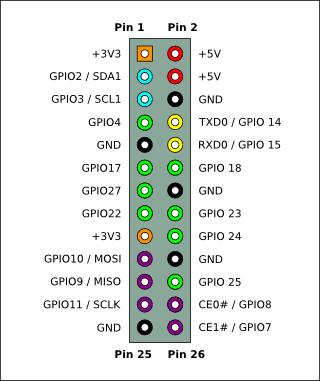
\includegraphics[scale=0.65]{latex_template_thesis_v4-2/Pi-GPIO-header-26-sm.png}
    \caption{The Raspberry Pi 1B GPIO pinout. Pins labeled \textit{GPIO \#} correspond to GPIO pins in the Broadcom BCM2835 peripherals manual\cite{bcm:2835peripherals}.}
    \label{fig:gpiopinout}
\end{figure}

\subsubsection{The VideoCore IV processor}
Coming from the x86 world, you might expect the VideoCore IV (VC4) GPU to be little more than a standard PC graphics card, managing and accelerating graphical output. While it certainly does do those things, the VC4 has much broader responsibilities on the Raspberry Pi. It runs a (real-time) operating system of its own, ThreadX\cite{rpi:opensourcevpu}, and handles system initialisation and the early boot process\cite{rpi:bootforum}. It also performs power and clock management\cite{rpi:gpuclockpower}. As described 

\chapter{My work}
\section{Porting \ucosiii to the Raspberry Pi}
To run \ucosiii on the Raspberry Pi, there needs to be a version of the operating system that has been adapted to run on the hardware the Pi uses. These adaptations are commonly called \textit{ports}. There are ports to architectures that are similar to that of the Pi, such as the ARM9-based NXP LPC2923 \cite{micrium:nxplpc}, but there is no port for the Broadcom BCM2835, the SoC used by the Pi. As mentioned in section~\ref{sec:ucos}, however, there is an extensive manual supplied with \ucosiii, which includes a chapter on porting it to different architectures. Additionally, a thesis has been written on porting \ucosii to the Pi\cite{sfd:realpi}, and there is a plethora of information available online on bare-metal programming on the Pi. Therefore, I decided porting \ucosiii would be an additional interesting, but doable challenge.

\subsection{The structure of \ucosiii}

\subsection{The components of a port}
When porting an operating system to a new platform, there are a number of components that need to be adapted. In the case of our \ucosiii port, the parts that need to be adapted are as follows.

\begin{itemize}
    \item Architectural features
    \item Interrupt handling
    \item Timers
    \item Serial I/O
\end{itemize}



\subsubsection{Architectural features}
In this part of the port, various features of the architecture are described. This consists of attributes such as the size of various data types, the availability of certain instructions and the modes of operation of certain features. More concretely, examples include:

\begin{itemize}
    \item The size of the processor's address bus.
    \item Whether the processor includes a count-leading-zeros instruction.
    \item Whether the processor stack grows upwards or downwards.
\end{itemize}

\subsubsection{Serial I/O} \label{sec:miniuart}
Implementing input/output capabilities is not strictly required to get \ucosiii running on the Raspberry Pi. An operating system is of little user without any I/O capabilities, however, and being able to output debugging information is also of great use in porting. 

The type of I/O that the port has support for is very common in embedded devices, and was used throughout much of the twentieth century for communication between computers and associated terminals: serial communication using a UART. The peripheral data sheet tells us that the Raspberry Pi contains two UARTs, a primary ARM PL011 UART and a secondary so-called `mini UART'. Our port uses the primary UART, as the baud rate of the secondary UART is linked to the VPU core frequency, which is variable by default, making the secondary UART `of limited use in the default state' \cite{rpi:uart}, and it has a number of other deficiencies described in \cite{bcm:2835peripherals}.

On the hardware side, the UART uses GPIO pins 8 and 10\footnote{Pin 14 and 15, respectively, in the Broadcom peripheral datasheet.} for transmit and receive, respectively. Additionally, one of the Pi's ground pins needs to be used to ensure the communicating devices have a common ground.

The process for setting up the UART can be split into a few parts. Firstly, the GPIO pins need to be set up to perform alternate function 0. Subsequently, the baud rate needs to be set

\subsubsection{Interrupts}
If, like me, you have spent some time playing around with bare-metal development on x86, you may be familiar with x86 interrupt handling. In brief: there are two programmable interrupt controllers, which are used to dispatch interrupts to the CPU. Devices hook into these controllers, and the controllers' interrupt masks can be programmed through software. When an interrupt arrives at the controller, it notifies the CPU by pulling the INTR pin high and sending it a corresponding IRQ number. The CPU then looks into an interrupt vector table, loads the handler address for a given IRQ number, and jumps to it. All of this is a luxury that the ARM architecture on the Pi does not offer us.

ARM uses the term `exception' to mean an event which causes the processor to stop execution and jump to a piece of code to handle it. The ARM architecture supports seven kinds of exceptions: \textit{Reset}, \textit{Undefined Instruction}, \textit{Software Interrupt}, \textit{Prefetch Abort}, \textit{Data Abort}, \textit{Interrupt} (IRQ) and \textit{Fast Interrupt} (FIQ). When an exception is generated, the CPU jumps to an \textit{exception vector} for the given exception. These vectors are usually located at the beginning of the address space, but can be remapped. An overview of exception types, their corresponding processor mode and address that execution starts at after exception reception is given in table~\ref{tbl:exceptions}.

\begin{table}[h]
    \centering
    \begin{tabular}{lll}
        \toprule
        \textbf{Exception type} & \textbf{Processor mode} & \textbf{Execution address} \\
        \midrule
        Reset & Supervisor & \texttt{0x00000000} \\
        Undefined instructions & Undefined & \texttt{0x00000004} \\
        Software interrupt & Supervisor & \texttt{0x00000008} \\
        Prefetch Abort & Abort & \texttt{0x0000000C} \\
        Data Abort & Abort & \texttt{0x00000010} \\
        IRQ (interrupt) & IRQ & \texttt{0x00000018} \\
        FIQ (fast interrupt) & FIQ & \texttt{0x0000001C} \\
        \bottomrule
    \end{tabular}
    \caption{An overview of ARM exceptions. Adapted from table A2-4 in the ARM Architecture Reference Manual\cite{arm:arm}.}
    \label{tbl:exceptions}
\end{table}

\subsubsection{Processor modes}
As well as jumping to a given address when an exception is generated, the processor changes its mode to one of the seven defined processor execution modes: \textit{User}, \textit{FIQ}, \textit{IRQ}, \textit{Supervisor} (SVC), \textit{Abort} (ABT), \textit{Undefined} (UND) and \textit{System} (SYS). These modes differ from each other in two important respects. Firstly, all modes except for user mode are privileged, i.e. can access all system resources, and can change mode freely.

\subsubsection{Timers}
Before the introduction of multi-core processors in the early 2000's, computing was largely a single-processor single-core affair (with notable exceptions dating back decades in the enterprise market). Despite this, multitasking was common even before the nineties. This is achieved through rapidly switching between tasks, letting the tasks appear to run in parallel. This switching can be done in cooperation with the tasks; this is  \textit{cooperative multitasking}, where tasks yield control to the operating system voluntarily to allow other tasks to run. This naturally causes problems when tasks do not yield, or do not yield often enough.

For that reason, cooperative multitasking has largely given way to \textit{pre-emptive} multitasking. In this paradigm, running tasks are periodically interrupted and control is transferred to the operating system, which decides whether the task should be \textit{switched out} so that another task may run, or should keep running. This periodic interruption is facilitated through a timer, which periodically generates a processor interrupt that transfers control to the operating system.

As described in the BCM2835 peripheral data sheet, the Raspberry Pi contains two timers; a timer for the ARM processor itself and a system timer. The ARM timer has issues similar to the `mini UART' described in section~\ref{sec:miniuart}, namely being dependent on the CPU core frequency


\subsubsection{Task switching}

\section{Implementing an adaptive scheduler}

\chapter{Experiments}

\chapter{Conclusions}

\printbibliography


\end{document}
